



Sea $U$ un conjunto y sea $A$ un subconjunto de $U$. Se llama
\semph{complementario} (o \emph{complemento}) de $A$ con respecto a $U$ al
conjunto de los elementos de $U$ que no pertenecen a $A$.

Existen varias notaciones para el complemento, como, por ejemplo,
$\complement_U A$. En muchas de estas, ni siquiera se especifica el conjunto
respecto al que se toma el complemento; habría que proporcionar esa
información en la prosa o quizás se sobrentienda. Esto último es lo más
usual. En ese caso, es normal encontrar las notaciones $\complement A$,
$A^\complement$, $A'$, $\overline{A}$, etc. Nosotros nos quedaremos con esta
última, ya que es bastante cómoda.

$$ \overline{A} = \{x \in U \st x \notin A\} $$

En el caso de que el conjunto $A$ esté definido por comprensión, como en

$$ A = \{x \in U \st P_x\} $$

\noindent se tendría que

$$ \overline{A} = \{x \in U \st \neg P_x\} $$

% TODO Ver si hay que poner elementos en el conjunto interior. Y poner
% referencia a la figura.

\begin{figure}
  \centering
  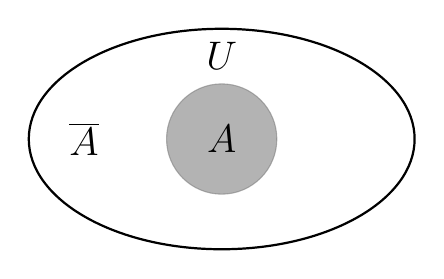
\begin{tikzpicture}[scale=0.7]
    % Dibujar el conjunto universal U como una elipse
    \draw[thick] (0,0) ellipse (3.5cm and 2cm);

    % Etiqueta del conjunto U
    \node at (0, 1.5) {\Large $U$};

    % Dibujar el conjunto A como un círculo más pequeño dentro de U
    \filldraw[opacity=0.6, black!50] (0,0) circle (1cm);

    % Etiqueta del complemento de A
    \node at (-2.5, 0) {\Large $\overline{A}$};

    % Etiqueta del conjunto A
    \node at (0, 0) {\Large $A$};

  \end{tikzpicture}
 \caption{Diagrama de Venn de $A$ y $\overline{A}$}
\end{figure}

\begin{example}
  Dado $U = \{a, b, c, d, 1, 2, 3, 4, 5, 6\}$, si $A = \{a, b, c, d\}$,
  entonces, $\overline{A} = \{1, 2, 3, 4, 5, 6\}$.

  Los complementarios respectivos de $\{0\}$ con relación a los conjuntos
  $\nset$, $\zset$, $\qset$ y $\rset$ se denotan usualmente como
  $\nset^{*}$, $\zset^{*}$, $\qset^{*}$ y $\rset^{*}$.

  En $\nset^{*}$, se tiene que el complementario del conjunto de números
  pares, es decir, de

  \[ P = \{x \in \nset^* \st x = 2k, \ k \in \nset^*\} = \{2k \st k \in
  \nset^*\} \]

  \noindent es el conjunto de los números impares:

  \[ \overline{P} = I = \{x \in \nset^* \st x = 2k - 1, \ k \in \nset^*\} =
  \{2k - 1 \st  k \in \nset^*\} \]
\end{example}

Consideremos todos los subconjuntos de un conjunto dado $A$. Forman un nuevo
conjunto que se denomina \semph{conjunto de las partes} (\emph{power set})
de $A$ y se designa por $\powset(A)$.

$$ \powset(A) = \{B \st B \subseteq A\} $$

Cualquiera que sea el conjunto $A$, se cumple que $\emptyset \in \powset(A)$
y $A \in \powset(A)$. La primera es lo mismo que se demostró para un
conjunto cualquiera; advierta que $\powset(A)$ es un conjunto. La otra
también es evidente ya que, para un conjunto $A$ cualquiera, se cumple $A
\subseteq A$.

Aunque $A$ sea el conjunto vacío, $A = \emptyset$, $\powset(A)$ no lo es
pues contiene a ese mismo conjunto como elemento, es decir, $\{\emptyset\}
\subseteq \powset(A)$.

\begin{example}
  Dado el conjunto con 4 elementos $A = \{a, b, c, d\}$, se tiene

  \begin{align*}
    \powset(A) =
    &\left\{ \emptyset, \{a\}, \{b\}, \{c\}, \{d\}, \{a, b\}, \{a, c\}, \{a,
      d\}, \{b, c\}, \{b, d\}, \{c, d\}, \{a, b, c\}, \right. \\
    &\left.\{a, b, d\}, \{a, c, d\}, \{b, c, d\}, A\right\} \\
  \end{align*}

  Si $A = \{a, b\}$, determine $\powset(A)$ y $\powset(\powset(A))$.

  \begin{align*}
    \powset(\powset(A)) =
    &\left\{
      \emptyset,
      \{\emptyset\},
      \{\{a\}\},
      \{\{b\}\},
      \{A\},
      \left\{\emptyset, \{a\}\right\},
      \left\{\emptyset, \{b\}\right\},
      \left\{\emptyset, A\right\},
      \left\{\{a\}, \{b\}\right\},
      \left\{\{a\}, A\right\},\right. \\
    &\left.\left\{\{b\}, A\right\},
      \left\{\emptyset, \{a\}, \{b\}\right\},
      \left\{\emptyset, \{a\}, A\right\},
      \left\{\emptyset, \{b\}, A\right\},
      \left\{\{a\}, \{b\}, A\right\},
      \powset(A)
    \right\} \\
  \end{align*}
\end{example}

\begin{example}
  Si el conjunto $A$ tiene $n$ elementos, ¿cuántos elementos tiene
  $\powset(A)$? Razone usando el Principio de Inducción.

  Se trata de un problema muy genérico, y, como tal, es un resultado
  importante de las matemáticas.

  % TODO Creo que está bastante desordenada.

  El proceso que vamos a seguir se basa en dividir el conjunto de las partes
  de un conjunto arbitrario $C$ en dos. Lo haremos tomando un elemento
  arbitrario $c \in C$. Tendremos, por un lado, los subconjuntos de $C$ que
  contienen a $c$, y, por el otro, los que no lo contienen. Ambos conjuntos
  serán disjuntos y su unión será igual que $\powset(C)$. De ahí,
  deduciremos una fórmula recursiva para $\card(\powset(C))$ y, luego, de
  esta deduciremos una fórmula explícita de $\card(\powset(C))$ en función
  de $\card(C)$.

  Tal y como hemos dicho, al conjunto arbitrario que tomaremos lo designamos
  por $C$. Por abreviar, al $\card(C)$ lo designaremos por $n$. También, al
  $\card(\powset(C))$ lo designaremos por $a_n$. Advierta que tiene que
  tener ese subíndice necesariamente.

  Veamos el caso base. Queremos que sea $n = 0$, por lo que tomamos $C =
  \emptyset$. Así, tal y como acabamos de decir, $n = \card(C) = 0$.
  También, se dará $a_0 = \card(\powset(C)) = 1$, ya que $\powset(\emptyset)
  = \{\emptyset\}$.

  Ahora, vamos al caso genérico. Suponemos que $C$ tiene $n$ elementos.
  Llamamos $D$ al subconjunto de $C$ cuando a este le quitamos un elemento
  arbitrario $c \in C$; es decir, $D = C \setminus \{c\}$. Se tiene que
  $\card(D) = n - 1$, como es evidente. Se tendrá entonces que
  $\card(\powset(C \setminus \{c\})) = \card(\powset(D)) = a_{n-1}$.

  % TODO Estoy usando la diferencia de conjuntos y se define después.

  Ahora, si a todo subconjunto de $D$, o, lo que es lo mismo, a todo $E \in
  \powset(C \setminus \{c\})$, le añadimos el elemento $c$, tendremos los
  mismos conjuntos que habríamos obtenido de haber seleccionado únicamente a
  los subconjuntos de $C$ que contienen al elemento $c$. Como los acabamos
  de construir a partir de $D$, el número de estos conjuntos será el mismo
  que los de aquel, es decir, $a_{n-1}$.

  Entonces, tenemos dos subconjuntos de $\powset(C)$ que son disjuntos entre
  sí y que cuya unión da $\powset(C)$. Como además, ambos tienen por tamaño
  $a_n$, se tendrá entonces que

  \[ a_n = a_{n-1} + a_{n-1} = 2 \, a_{n-1} \]

  Tenemos entonces la fórmula en forma recursiva de $a_n$. Esta es:

  \begin{equation*}
    a_n
    \begin{cases}
      1             & \text{si} \ n = 0 \\
      2 \, a_{n-1}  & \text{si} \ n > 0
    \end{cases}
  \end{equation*}

  A la vista de lo siguiente,

  \[ a_n = 2\, a_{n-1} = 2 (2\, a_{n-2}) = 2 (2 (2\, a_{n-3})) = \cdots = 2
  (2 (2 (2\, \cdot \cdots \cdot (2\, a_0)))) \]

  \noindent tiene pinta que la fórmula explícita será la siguiente:

  \[ a_n = a_0 \, \prod_{i=0}^n 2 = 1 \cdot 2^n = 2^n \]

  \noindent pero esto no lo hemos demostrado. Aquí es cuando haremos uso del
  Principio de Inducción. El caso base se dará para el valor $n = 0$. Para
  este se tiene que $a_0 = 1$.

  Ahora, pasamos a ver la hipótesis de inducción. Será

  \[ a_n = 2^n \]

  La meta de inducción será

  \[ a_{n+1} = 2^{n+1} \]

  Vamos a ver si de la hipótesis se deduce la meta. Tenemos que, aplicando
  la definición recursiva, se tiene

  \[ a_{n+1} = 2 \, a_n = 2 \cdot 2^n = 2^{n+1} \]

  \noindent que es a donde queríamos llegar. Así, hemos demostrado que la
  fórmula explícita de $a_n$ es

  \[ a_n = 2^n \]

  Con esto hemos demostrado que

  \[ \card(\powset(C)) = 2^{\card(C)} \]

  Existen otras demostraciones alternativas. Por ejemplo, haciendo uso de la
  combinatoria.
\end{example}




